\documentclass[tikz]{standalone}
\usepackage[outline]{contour}

\begin{document}
	    \contourlength{1.2pt}
	    
	    \tikzset{
	    	double arrow/.style args={#1 colored by #2 and #3}{
	    		-stealth,line width=#1,#2, % first arrow
	    		postaction={draw,-stealth,#3,line width=(#1)/3,
	    			shorten <=(#1)/3,shorten >=2*(#1)/3}, % second arrow
	    	}
	    }
\begin{tikzpicture}
    \node[anchor=south west,inner sep=0] at (0,0) {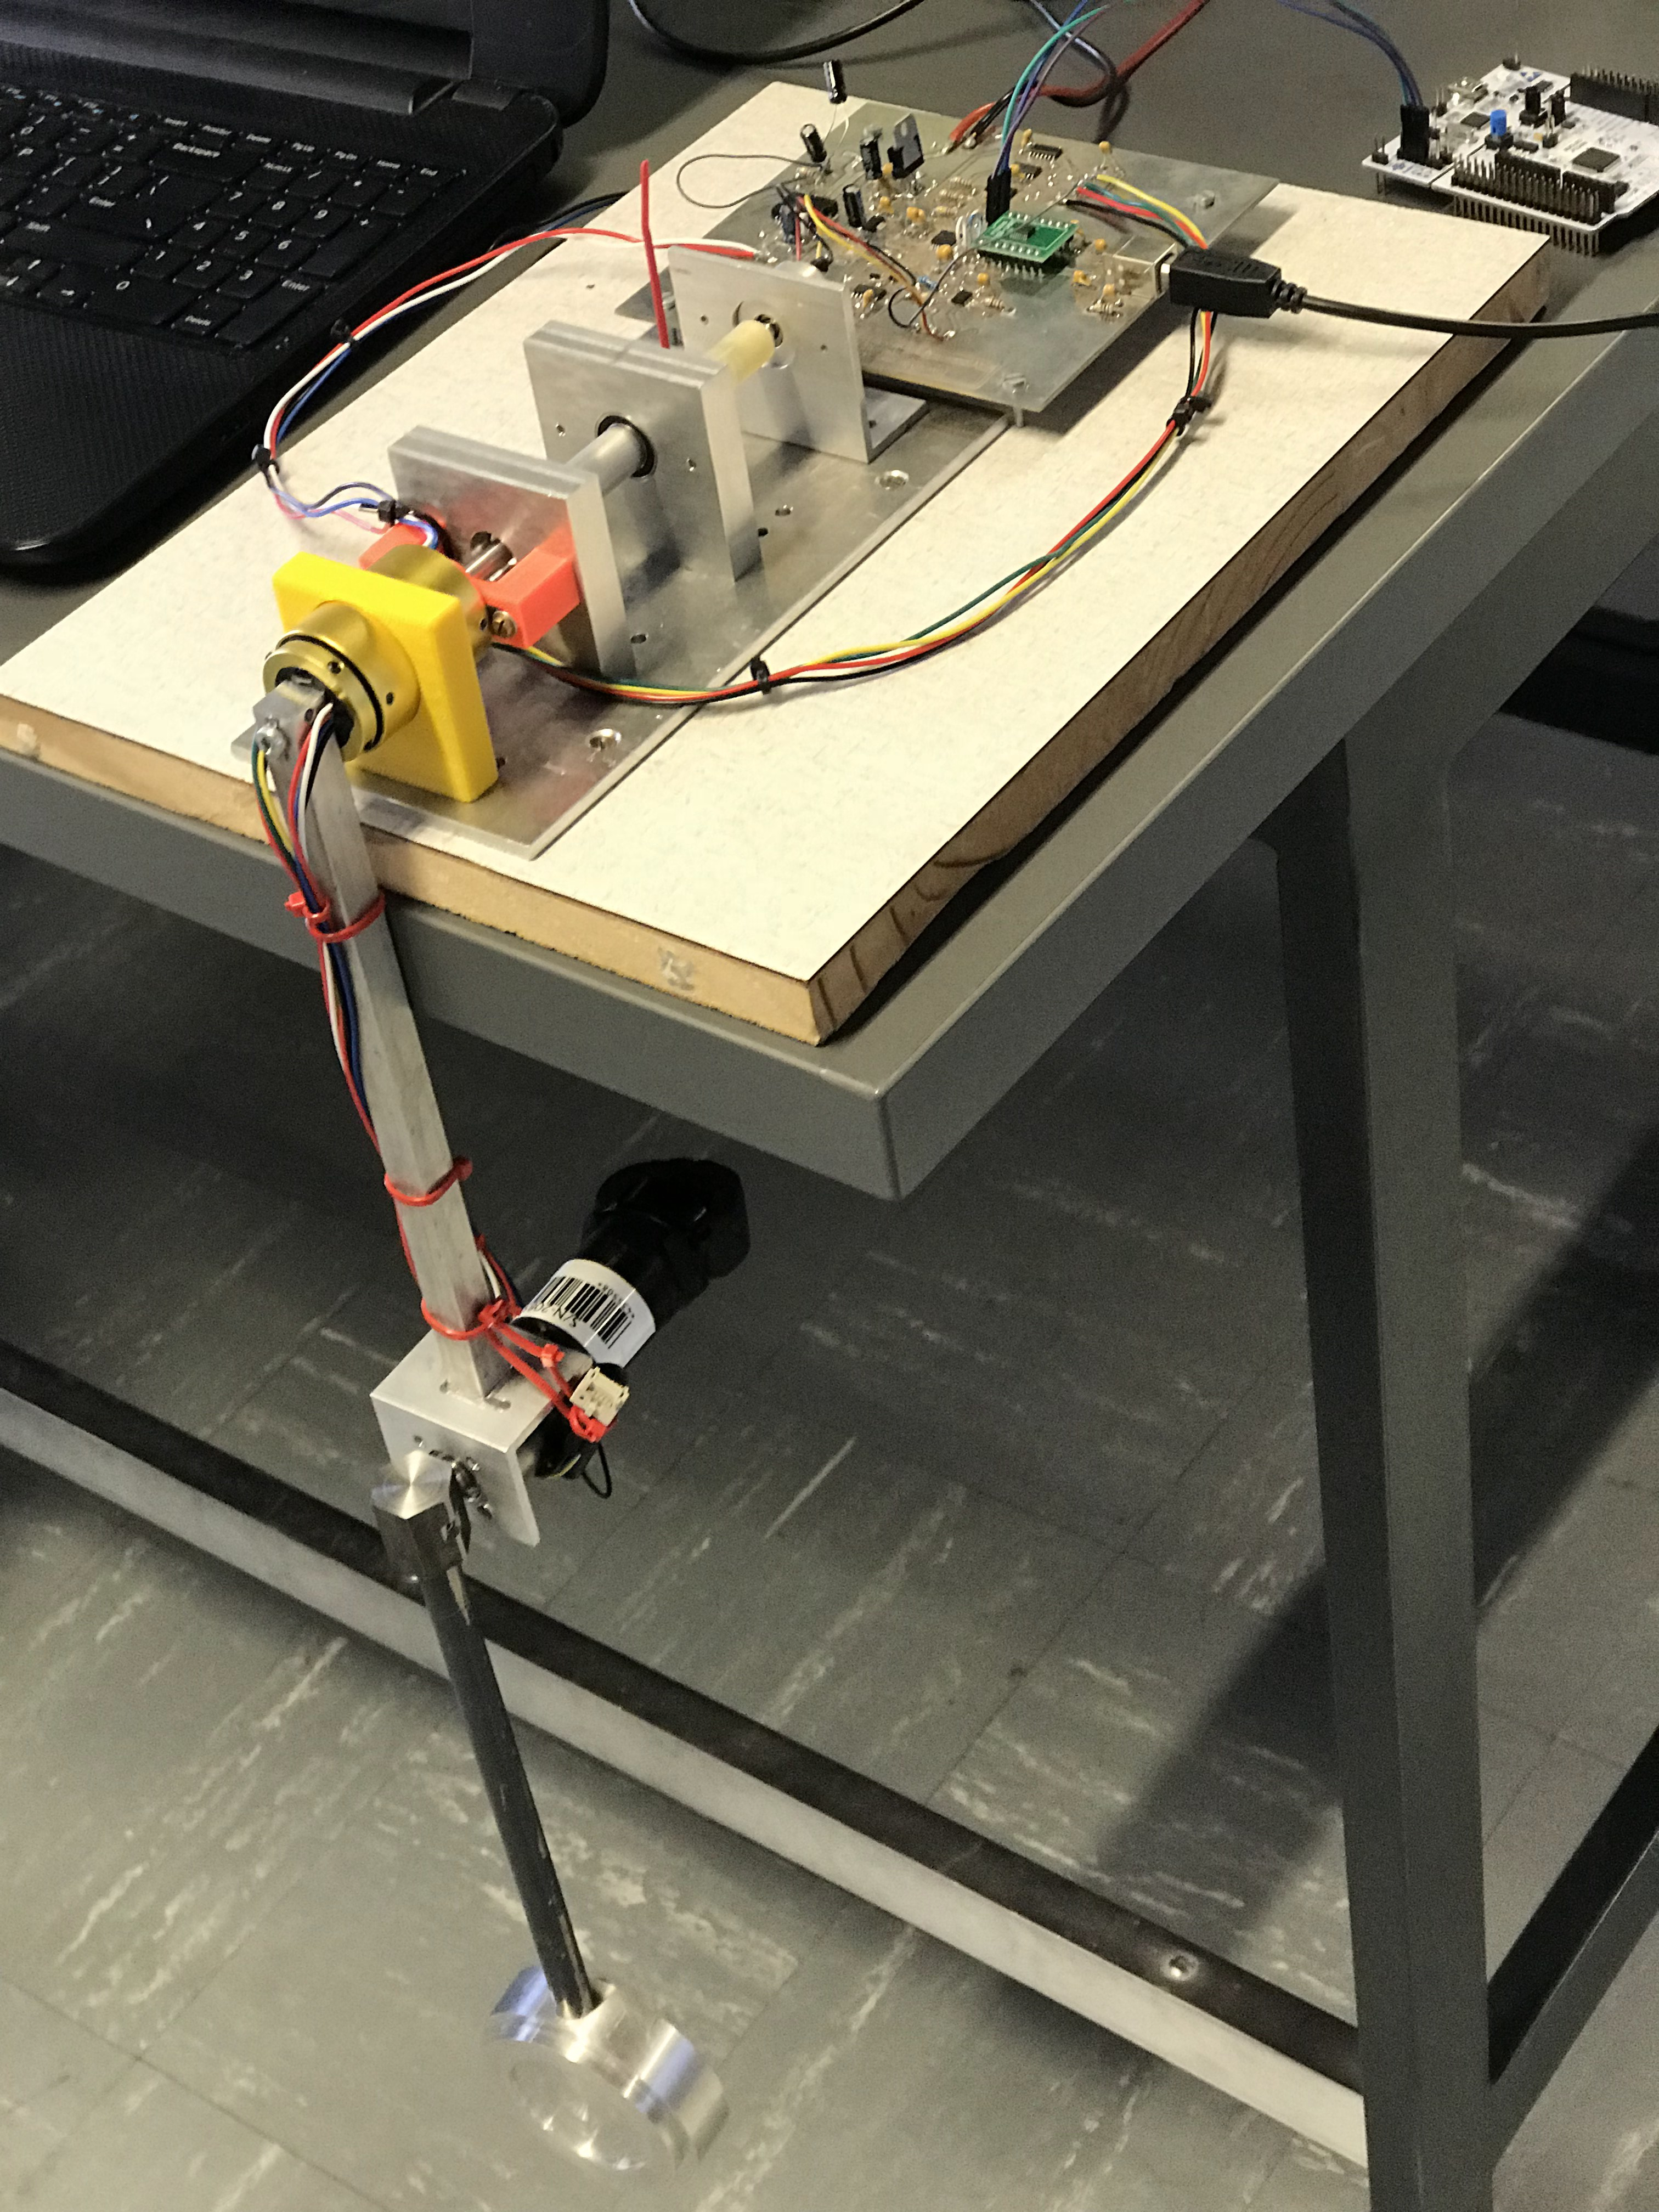
\includegraphics[width=\textwidth]{mech.jpg}};
    %microcontroller
    %\draw[green,ultra thick,rounded corners] (6.5,5) node[above]{ \textbf{MCU} };
    
	\draw[double arrow=2pt colored by black and white] (8,2) node[right,white]{\contour{black}{Point Mass} } -- (4.5,0.8) ;
	
	\draw[black,thick,->] (3.8,3) -- (8,3) node[right,white]{\contour{black}{Actuated Pendulum}};
	
	\draw[black,thick,->] (3.8,6) -- (8,4) node[right,white]{\contour{black}{Motor Mounting}};
	
	\draw[black,thick,->] (4.5,6.5) -- (8,5) node[right,white]{\contour{black}{DC Motor}};
	
	\draw[black,thick,->] (5,7) -- (8,6) node[right,white]{\contour{black}{Encoder}};
    
    \draw[black,thick,->] (2.8,9) -- (8,7) node[right,white]{\contour{black}{Unactuated Pendulum}};
    
    \draw[black,thick,->] (2.8,11) -- (8,8) node[right,white]{\contour{black}{Slipring}};
    
    \draw[black,thick,->] (3.5,12.5) -- (8,9) node[right,white]{\contour{black}{Bearing Housing}};
    
    \draw[black,thick,->] (4.4,12.8) -- (8,10) node[right,white]{\contour{black}{Shaft}};
    
    \draw[black,thick,->] (5.5,13.5) -- (8,11) node[right,white]{\contour{black}{Rubber Coupling}};
    
    \draw[black,thick,->] (5.8,14.2) -- (8,12) node[right,white]{\contour{black}{Potentiometer}};
    
    
\end{tikzpicture}
\end{document}